\documentclass[12pt]{article}
\usepackage[utf8]{inputenc}
\usepackage[english]{babel}
\usepackage[letterpaper, portrait, margin=1in]{geometry}
\usepackage{amsmath}
\numberwithin{equation}{section}
\usepackage{amssymb}
\usepackage{graphicx}
\usepackage{parskip}
\usepackage{xcolor}
\usepackage{physics}
\usepackage{empheq}
\usepackage{cancel}
\usepackage{hyperref}
\hypersetup{colorlinks = true, urlcolor = blue, linkcolor = red, citecolor = red}
\usepackage{enumerate}
\usepackage{tikz}
\usepackage{float}
\usepackage{tcolorbox}
\usepackage{booktabs}
\usepackage[bottom]{footmisc}

% Default fixed font does not support bold face
\DeclareFixedFont{\ttb}{T1}{txtt}{bx}{n}{12} % for bold
\DeclareFixedFont{\ttm}{T1}{txtt}{m}{n}{12}  % for normal

% Custom colors
\usepackage{color}
\definecolor{deepblue}{rgb}{0,0,0.5}
\definecolor{deepred}{rgb}{0.6,0,0}
\definecolor{deepgreen}{rgb}{0,0.5,0}

\usepackage{listings}

% Python style for highlighting
\newcommand\pythonstyle{\lstset{
		language=Python,
		basicstyle=\ttm,
		morekeywords={self},              % Add keywords here
		commentstyle=\color{gray},
		keywordstyle=\ttb\color{deepblue},
		emph={MyClass,__init__},          % Custom highlighting
		emphstyle=\ttb\color{deepred},    % Custom highlighting style
		stringstyle=\color{deepgreen},                        % Any extra options here
		showstringspaces=false
}}


% Python environment
\lstnewenvironment{python}[1][]
{
	\pythonstyle
	\lstset{#1}
}
{}

% Python for external files
\newcommand\pythonexternal[2][]{{
		\pythonstyle
		\lstinputlisting[#1]{#2}}}

% Python for inline
\newcommand\pythoninline[1]{{\pythonstyle\lstinline!#1!}}

\usepackage{xcolor}
\usepackage{fancyhdr}
\pagestyle{fancy}
\fancyhf{}
\fancyfoot[C]{\color{lightgray} Python Lecture II Notes}
\fancyfoot[L]{\color{lightgray} \today}
\fancyfoot[R]{Page \thepage}
\renewcommand{\headrulewidth}{0pt}
\renewcommand{\footrulewidth}{0pt}


\begin{document}

\vspace*{-2.5cm}{\footnotesize\hfill Copyright \copyright\the\year{} Yi J Zhu}
\section{Review}


\textbf{Last time:}
\begin{itemize}
    \item The kernel is the program at the ``heart" of your computer. It is the first program to start when your computer boots and interfaces between the hardware and software.
    \item We can interact with the kernel via the OS (GUI) or shell (text terminal/command line).
    \item Two steps for programming in Python. (1) Write Python code (which is just text) and (2) Use a program called the interpreter to execute the code.
    \item IDE: allows us to write and execute code using one all-inclusive program (i.e. with a single button click).
\end{itemize}

\section{Python on the Terminal}
\textbf{Demo:} you can interact directly with the python interpreter from the command line. Demo print statement, math. (cltr-d to quit).

What's happening: you're writing code in the terminal and sending it the interpreter to execute when you press enter.

\textbf{Demo:} you can also run a .py file from the command line with the python command. 

Here, we're invoking the interpreter and telling it to execute the file we're specifying rather than starting an interactive session (before).

\textbf{This process is not ideal}

\begin{itemize}
    \item Have to save the .py file every time you make a change
    \item Have to type a command on the terminal (different window) every time you want to run a piece of code
    \item What if your program outputs something other than text, e.g. plots. Terminal does not handle it elegantly...
    \item We're going to solve this problem in the next section
\end{itemize}

\section{Jupyter Notebook}
\textbf{Q: What is Anaconda?}
\begin{itemize}
    \item NOTE: Students should have downloaded Anaconda before lecture. Make sure Anaconda is added to PATH!
    \item Anaconda is a distribution of PYTHON with some additional software. 
    \item One such software we're interested in is Jupyter notebook
    \item Anaconda is also popular in research because people can share packages with Conda
\end{itemize}

\textbf{Q: What is Jupyter notebook?}
\begin{itemize}
    \item Jupyter is an IDE. There are other IDEs!
    \item \textbf{Demo (students follow along):} open Jupyter notebook from the command-line.
    \item Jupyter starts a server and you interact with it's GUI via a browser. (Not important for you to understand, but that's why you're using a web browser)
    \item Demo: creating new notebook.
    \item Jupyter notebook files has for .ipynb (ipython notebook)
    \item Jupyter is organized by cells. You can run code in each cell independent of other cells.
    \item Jupyter has code cells and markdown cells where we can type text/math/images
    \item To run cell: shift-enter
    \item To enter command mode: press esc. (The  cell is surrounded by a green in edit mode and blue in command mode). In command mode ``dd" to delete cell, ``A" to add cell above, and ``B" to add cell below.
    \item Jupyter notebooks have a kernel. This ``kernel" does not have the same meaning as what we discussed last lecture. Think ``kernel"$=$``Python interpreter"
    \item Jupyter default autosave interval: 120 seconds
\end{itemize}

\section{Python Intro}
\textbf{Syntax:}
\begin{itemize}
    \item Python is case-sensitive and indentation sensitive
    \item Comments: hash symbol for single line comment. Triple quotes (""") surrounding multi-line comment
\end{itemize}

\textbf{Variables:}
\begin{itemize}
    \item Containers for storing data we want to keep track of
    \begin{figure}[H]
	    \centering
	    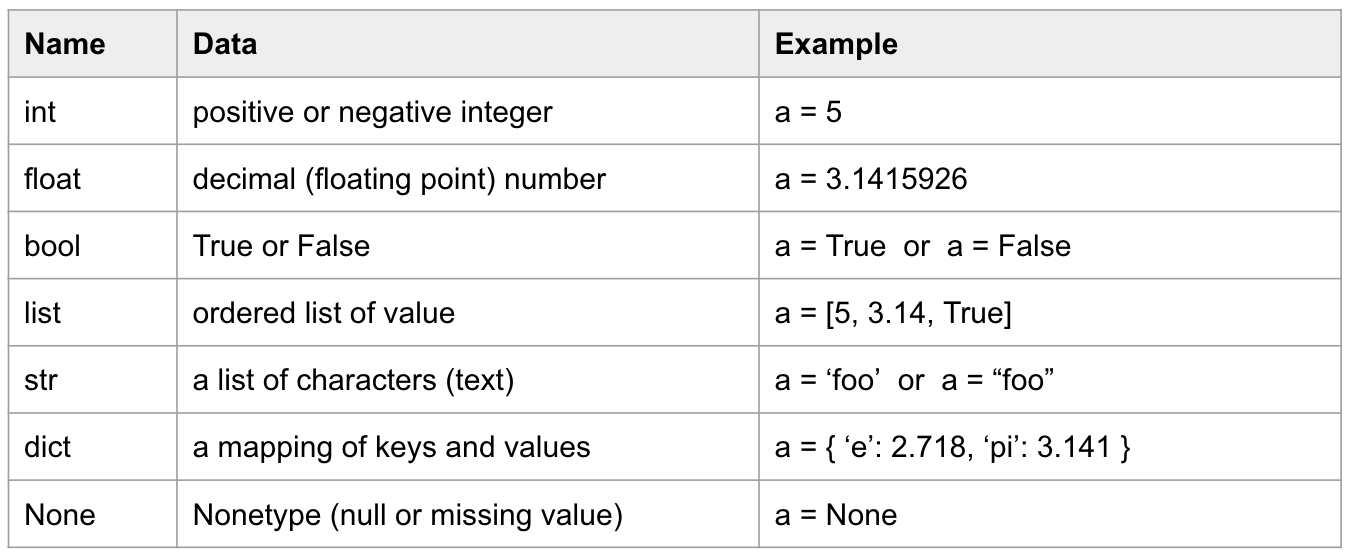
\includegraphics[height=4.8cm] {data}
\end{figure}
    \item Demo: We can determine the data type with the type() function
\end{itemize}

\textbf{Dynamic typing}
\begin{itemize}
    \item We do not have to specify the type of variable beforehand.
    \item We can change the type of data that a variables stores easily. \textbf{Demo: }$a=5, a=$`foo'
    \item Convenient, but sometimes causes issues when the type of variable is not what you or the compiler expected.
    \item To create a variable, just assign it a value
    \item Casting: specifying the type that a variable should be. \textbf{Demo:}
    \begin{figure}[H]
	    \centering
	    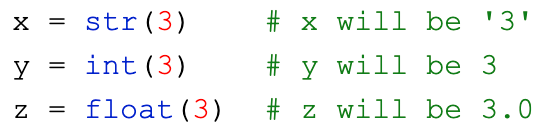
\includegraphics[width=7cm] {cast}
    \end{figure}
    \item Be careful when casting floats to ints. \textbf{The float constructor does not round, it throws away the decimal.}
\end{itemize}

\textbf{Demo: Printing variables}
\begin{itemize}
    \item print statement: \verb|print('hi')|
    \item concatenate strings: \verb|name=`ulab'; print(`hi ' + name)|
    \item What happens when? \verb|age=5; print(`age is ' + age)|. Demo: reading stacktrace. We need to cast!
    \item String formatting: \verb|`my name is {} and I am {} years old'.format({'ulab'}, {5})|. You can read up on more advance formatting operations
\end{itemize}

\textbf{Mathematical operations:}
\begin{figure}[H]
	\centering
	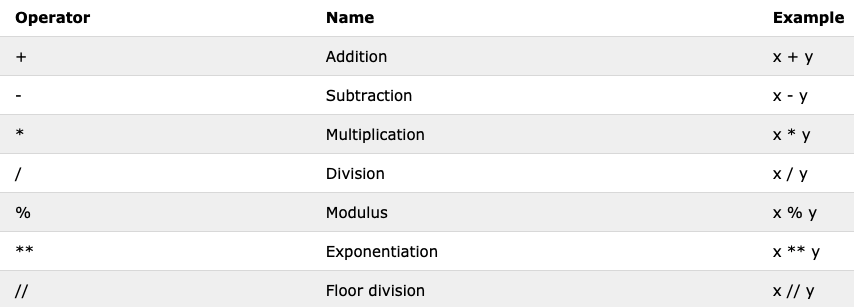
\includegraphics[width=15cm] {math}
\end{figure}

\textbf{Comparison operations: }
\begin{figure}[H]
	\centering
	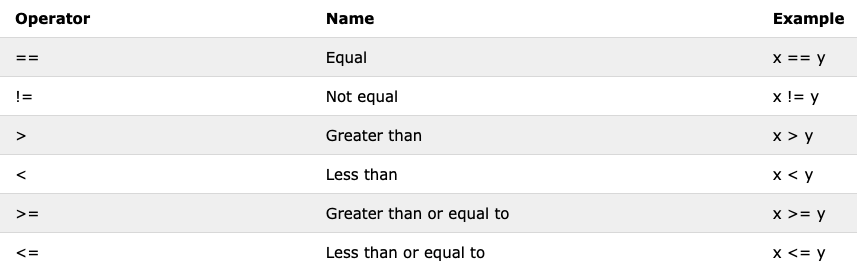
\includegraphics[width=15cm] {comp}
\end{figure}
Explain: we use == rather than = because = is used to assign values.

\textbf{Logic operations: }
\begin{figure}[H]
	\centering
	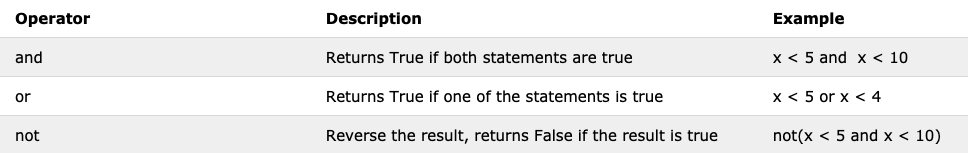
\includegraphics[width=15cm] {logic}
\end{figure}

\section{Lists}
\begin{itemize}
    \item Lists are ordered and zero indexed
    \begin{figure}[H]
	    \centering
	    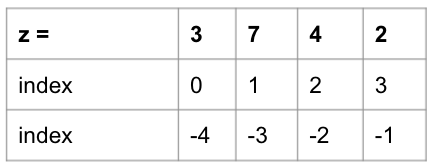
\includegraphics[width=6cm] {index}
    \end{figure}
    \item Reminder: elements do not have to be the same type: \verb| z = [`ulab', 5]|
    \item Access element: \verb| name = z[0]|
    \item Change element: \verb|z[1] = z[1] + 1|
    \item Length of a list: \verb|len(z)|
    \item Create an empty list: \verb|z = []|
\end{itemize}

\textbf{More about lists:}
\begin{itemize}
    \item Negative indexing: index of -1 is the last element of the list. Counting down indexes from back to front.
    \item Slicing: [start : end : jump]. Demo: \verb|z[1:3], z[:], z[1:], z[:3], z[::2], z[-2:-1]|
    \item List methods: append(), extend(), index(), more but we use these three the most.
\end{itemize}

\section{Conditionals}
We use conditionals when we want a block of code to run IF some CONDITION is true.
\begin{itemize}
    \item Demo: single if block
    \item Demo: if else block
    \item Demo: if elif else block
    \item Demo: if elif elif ... elif else block
    \item Notice: the program exits the loop IF an \verb|if| or \verb|elif| block is executed. Subsequent \verb|elif| or \verb|else| blocks (if there are any) are ignored.
\end{itemize}

\section{Next Week}
\begin{itemize}
    \item Loops, functions, more Python!
\end{itemize}

\section{Homework}
\begin{itemize}
    \item For the most part HWs from now on will be in Jupyter notebook. Demo: saving notebook as PDF.
    \item Practice with Jupyter, variables, math, lists, and conditionals
\end{itemize}

\appendix
\section{(Optional) String Formatting}

\textbf{Formatting text}: \pythoninline{print('pi is {}'.format(math.pi))}

A useful list of options for formatting numbers:

\begin{table}[H]
	\begin{tabular}{l | l | l | l}
		\textbf{Number} & \textbf{Format}            & \textbf{Output} & \textbf{Description}                          \\
		\hline
		3.1415926       & \{:.2f\}                   & 3.14            & Format float 2 decimal places                 \\
		3.1415926       & \{:+.2f\}                  & +3.14           & Format float 2 decimal places with sign       \\
		-1              & \{:+.2f\}                  & -1.00           & Format float 2 decimal places with sign       \\
		2.71828         & \{:.0f\}                   & 3               & Format float with no decimal places           \\
		5               & \{:0\textgreater{}2d\}     & 05              & Pad number with zeros (left padding, width 2) \\
		5               & \{:x\textless{}4d\}        & 5xxx            & Pad number with x’s (right padding, width 4)  \\
		10              & \{:x\textless{}4d\}        & 10xx            & Pad number with x’s (right padding, width 4)  \\
		1000000         & \{:,\}                     & 1,000,000       & Number format with comma separator            \\
		0.25            & \{:.2\%\}                  & 25.00\%         & Format percentage                             \\
		1000000000      & \{:.2e\}                   & 1.00e+09        & Exponent notation                             \\
		13              & \{:10d\}                   & 13              & Right aligned (default, width 10)             \\
		13              & \{:\textless{}10d\}        & 13              & Left aligned (width 10)                       \\
		13              & \{:\textasciicircum{}10d\} & 13              & Center aligned (width 10)                    
	\end{tabular}
\end{table}

\textbf{We can substitute multiple variables:}
\begin{python}
s1 = "cats"
s2 = "dogs"
s3 = " it's raining {} and {} ".format(s1, s2)

>>> s3
"it's raining cats and dogs"
\end{python}

\textbf{Using numbered parameters:}
\begin{python}
s = "{0}: Oh {1}, {1}! Wherefore art thou {1}?".format("Juliet", "Romeo")

>>> s
'Juliet: Oh Romeo, Romeo! Wherefore art thou Romeo?'
\end{python}

\textbf{F-Strings:}
\begin{python}
book = "Lord of the Rings"
author = "J.R.R. Tolkien"
s = f"The {book} was written by {author}" 

>>> s
'The Lord of the Rings was written by J.R.R. Tolkien'
\end{python}

\end{document}
